
\documentclass[9pt]{extarticle}
\usepackage[margin=0.7cm]{geometry}
\usepackage[UKenglish]{babel}
\usepackage{parallel,enumitem}
\usepackage{multicol}
\setlength{\columnsep}{0.7cm}
\setlength{\columnseprule}{0.5pt}
\usepackage{amssymb}
\usepackage{amsmath}
\usepackage{bm}
\usepackage{graphicx}
\graphicspath{{./pics/}}
\usepackage{physics}

%% vectors and matrices
\renewcommand{\v}[1]{{\bm #1}}
\renewcommand{\dv}[1]{\dot{\bm{#1}}}
\newcommand{\ddv}[1]{\ddot{\bm{#1}}}
\newcommand{\hv}[1]{\hat{\bm{#1}}}
\newcommand{\m}[1]{[ #1 ]}
\renewcommand{\t}[1]{\widetilde{\bm{#1}}}
\newcommand{\bfit}[1]{\textbf{\textit{#1}}}

%% differential and integral operators
\renewcommand{\d}{\text{d}}
\renewcommand{\dd}[2]{\frac{\d #1}{\d #2}}
\newcommand{\ddd}[2]{\frac{\d^2 #1}{\d #2^2}}
\newcommand{\ddt}[1]{\frac{\d #1}{\d t}}
\newcommand{\dddt}[1]{\frac{\d^2 #1}{\d t^2}}
\newcommand{\pd}[2]{\frac{\partial #1}{\partial #2}}
\newcommand{\pdd}[2]{\frac{\partial^2 #1}{\partial #2^2}}
\renewcommand{\grad}{\boldsymbol \nabla} 
\renewcommand{\div}{\boldsymbol \nabla \cdot}
\renewcommand{\curl}{\boldsymbol \nabla \times}
\newcommand{\lap}{\nabla^2}
\newcommand{\intinf}{\int_{-\infty}^\infty}
\newcommand{\intzinf}{\int_0^\infty}
\newcommand{\intinfz}{\int_{-\infty}^0}

%% constants
\newcommand{\eo}{\epsilon_0}
\newcommand{\muo}{\mu_0}

%% statistics
\newcommand{\E}{\text{E}}
\newcommand{\Var}{\text{Var}}
\newcommand{\SD}{\text{SD}}
\newcommand{\SE}{\text{SE}}
\newcommand{\Cov}{\text{Cov}}
\newcommand{\Cor}{\text{Cor}}
\renewcommand{\P}{\text{P}}
\newcommand{\Bias}{\text{Bias}}

\begin{document}

\setlength{\parindent}{0pt}

{\huge \bf problem set} 

\noindent \hrulefill

\begin{multicols*}{2}

{\LARGE \bf I --- Superluminal Motion in Astronomy} \\

{\it Griffiths 12.6} \\ 

Every two years, more or less, the {\it NYT} publishes an article in which some astronomer claims to have found an object travelling faster than the speed of light. Many of these reports result from a failure to distinguish what is {\it seen} from what is {\it observed}---that is, from a failure to account for light travel time. Here's an example: a star is travelling with speed $v$ at an angle $\theta$ to the line of sight. What is its apparent speed across the sky? Suppose the light signal from $b$ reaches the earth at a time $\Delta t$ after the signal from $a$, and the star has meanwhile advanced a distance $\Delta s$ across the celestial sphere; by ``apparent speed," I mean $\Delta s / \Delta t$. What angle $\theta$ gives the maximum apparent speed? Show that the apparent speed can be much greater than $c$, even if $v$ itself is less than $c$. \\ 

{\bfit{Solution}} \\ 

Define $t_a'$ to be the time the light signal leaves $a$, and $t_a$ to be the time it arrives on earth, and $d_a$ to be the distance travelled by the signal between point $a$ and the earth. Likewise define $t_b'$, $t_b$, and $d_b$ as the equivalent variables concerning point $b$.  \\ 

The observed time difference, $\Delta t$, is $\Delta t = t_b - t_a$, where:

$$t_a = t_a' + \frac{d_a}{c}$$
$$t_b = t_b' + \frac{d_b}{c}$$ \ 

Using this, the observed time difference can be expressed:

$$
\begin{aligned}
	\Delta t &= t_b - t_a = t_b' - t_a' - \frac{d_b-d_a}{c} \\  
	&= \Delta t' - \frac{v\cos\theta \Delta t'}{c} \\ 
	&= \Delta t' \bigg(1 - \frac{v\cos\theta}{c} \bigg)
\end{aligned}
$$ \ 

where $\Delta t' = t_b' - t_a'$. \\

The observed distance $\Delta s$ can be expressed:

$$\Delta s = v\sin\theta \Delta t'$$ \ 

And, thus, the observed speed $u$ is:

$$u = \frac{\Delta s}{\Delta t} = \frac{v\sin\theta \Delta t'}{\Delta t' \big( 1 - \frac{v\cos\theta}{c} \big)} = \frac{v\sin\theta}{1-\frac{v\cos\theta}{c}}$$ \ 

The angle $\theta$ that gives the maximum observed speed can be found by setting $\dd u \theta = 0$, as follows:

$$\dd u \theta = \frac{v \big[ (1-\tfrac vc \cos\theta)(\cos\theta) - \sin\theta(\tfrac vc \sin\theta) \big]}{(1-\tfrac vc \cos\theta)^2} = 0$$ \ 

which gives:

$$\Longrightarrow \;\; (1-\tfrac vc \cos\theta)\cos\theta = \tfrac vc \sin^2\theta$$

$$\Longrightarrow \;\; \cos\theta = \frac vc (\sin^2\theta + \cos^2\theta) = \frac vc$$ \ 

Thus:

$$\theta_{\text{max}} = \cos^{-1} \bigg(\frac vc \bigg)$$ \ 

At this angle, the observed speed is:

$$u_{\text{max}} = \frac{v\sin(\cos^{-1}(\tfrac vc))}{1-\tfrac vc \cos(\cos^{-1}(\tfrac vc))} = \frac{v\sqrt{1-v^2/c^2}}{1-v^2/c^2} = \frac{v}{\sqrt{1-v^2/c^2}}$$ \ 

Note that as $v \rightarrow c$, the denominator goes to zero, meaning the observed speed $u$ can get infinitely large even as the actual speed $v$ is smaller than $c$. \\ 







\hrulefill 

\hfill 

{\LARGE \bf II --- Alternate Universe} \\ 

{\Large \bf a.} Imagine that in another universe the speed of light is only $c=100$ m/s. A person travelling along an interstate highway at 120 km/h ages how much slower than a person at rest? \\ 

{\bfit{Solution}} \\ 

120 km/h is $120 \cdot \frac{1000}{3600} = 33.33$ m/s. \\ 

The ratio of the change in time in the rest frame to that in the moving frame is given by the quantity $\gamma$:

$$\frac{\Delta t}{\Delta t'} = \frac{1}{\sqrt{1-v^2/c^2}} = \gamma$$ \ 

In this case this ratio is:

$$\gamma = \frac{1}{\sqrt{1-33.33^2/100^2}} = 1.0606$$ \ 

Thus in the moving frame, the person ages approximately 1.06 times more slowly that in the rest frame. \\ 




\dotfill 

\hfill 

{\Large \bf b.} Given the same universe as in part a, an airplane 40 m long at rest and which flies at 300 km/h will appear to be how long to an observer at rest? \\ 

{\bfit{Solution}} \\ 

300 km/h is $300 \cdot \frac{1000}{3600} = 83.33$ m/s. \\ 

In this case $\gamma$ is:

$$\gamma = \frac{1}{\sqrt{1-83.33^2/100^2}} = 1.809$$ \

In the moving frame, $\Delta x' =  \gamma \Delta x$, meaning:

$$\Delta x = \frac{\Delta x'}{\gamma} = \frac{40}{1.809} = 22.11$$ \

Thus, to the observer at rest, the plane will appear to be only 22.11 m long.  





\hrulefill 

\hfill 

{\LARGE \bf III --- Golf Diplomacy} \\ 

A mechanism on earth useed to shoot down geosynchronous satellites that house laser-based weapons is finally perfected and propels golf balls at speeds of $0.94c$. \\ 

{\Large \bf a.} How far will a detector riding with the golf ball initially measure the distance to the satellite? Note geosynchronous satellites are placed $3.58 \cdot 10^4$ km  above the surface of the earth. \\ 

{\bfit{Solution}} \\ 

In this case $\gamma$ is:

$$\gamma = \frac{1}{\sqrt{1-0.94^2}}  = 2.931$$ \ 

The detector will measure a distance to the satellite:

$$d = \frac{d'}{\gamma} = \frac{3.58 \cdot 10^4}{2.931} = 1.221 \cdot 10^4$$ \ 

i.e. the detector will measure a distance of approximately 1221 km. \\ 




\dotfill 

\hfill 

{\Large \bf b.} How much time will it take the golf ball to make the journey to the satellite in the earth's frame? How much time will it take in the golf ball's frame? \\ 

{\bfit{Solution}} \\ 

In the earth's frame, it will take:

$$t = \frac{3.58\cdot 10^4}{0.94 \cdot (3 \cdot 10^8)} = 0.00012695 \; \text{s}$$ \ 

i.e. approximately 127 $\mu$s. \\ 

In the golf ball's frame, it will take:

$$t = \frac{1221}{0.94 \cdot (3 \cdot 10^8)} = 0.0000043298 \; \text{s}$$ \

i.e. approximately 4.33 $\mu$s. \\ 






\hrulefill 

\hfill 

{\LARGE \bf IV --- Time Dilation} \\ 

{\Large \bf a.} Astronomers discover a planet orbiting around a star similar to our sun that is 20 light years away. How fast must a rocket ship go if the round trip is to take no longer than 40 years in time for the astronauts aboard? How much time will the trip take on earth? \\ 

{\bfit{Solution}} \\ 

The Lorentz contraction formula:

$$\Delta x' = \frac{1}{\sqrt{1-v^2/c^2}} \Delta x$$ \ 

where $\Delta x = v \Delta t$. Substituting this, and rearranging:

$$
\begin{aligned}
	\Delta x' &= \frac{1}{\sqrt{1-v^2/c^2}} v \Delta t \\ 
	1-\frac{v^2}{c^2} &= \frac{1}{(\Delta x)^2} (\Delta t)^2 \\ 
	\frac{1}{v^2} &= \frac{1}{(\Delta x)^2} (\Delta t)^2 + \frac{1}{c^2} \\ 
	v^2 &= \frac{1}{\frac{(\Delta t)^2}{(\Delta x')^2} + \frac{1}{c^2}} \\ 
	&= \frac{1}{\frac{(40\text{y})^2}{(40\text{ly})^2} + \frac{1}{c^2}} \\ 
	&= \frac{1}{\frac{1}{c^2} + \frac{1}{c^2}} \\ 
	&= \frac{c^2}{2}
\end{aligned}
$$ \ 

$$\therefore \;\; v = \frac{1}{\sqrt 2}c$$ \ 

The time taken on earth is given by the time dilation formula:

$$\Delta t' = \frac{1}{\sqrt{1-v^2/c^2}} \Delta t = \frac{40}{\sqrt{1 - \big( \tfrac{1}{\sqrt 2} \big)^2}} = 56.57$$ \ 

Thus it will take approximately 56.57 years on earth. \\ 






\dotfill 

\hfill 

{\Large \bf b.} Particle physicists use particle track detectors to determine the lifetime of short-lived particles. A muon has a mean lifetime of 2.2 $\mu$s and makes a track 950 m long before decaying into an electron and two neutrinos. What was the speed of the muon? \\ 

{\bfit{Solution}} \\ 

Using the same expression from part a, the speed of the muon is given by:

$$v = \sqrt{\frac{1}{\frac{(\Delta t)^2}{(\Delta x')^2} + \frac{1}{c^2}}}$$ \ 

where $\Delta t$ is the time taken in the muon's frame and $\Delta x'$ is the distance travelled in the lab frame. Substituting 2.2 $\mu$s and 950 m gives:

$$v = \sqrt{\frac{1}{\frac{(2.2\cdot 10^{-6})^2}{950^2} + \frac{1}{(3 \cdot 10^8)^2}}} = 2.464 \cdot 10^8$$ \ 

i.e. the speed of the muon was $2.464 \cdot 10^8$ m/s or 0.821$c$. \\ 



 





\hrulefill 

\hfill 

{\LARGE \bf V --- Length Contraction} \\ 

{\Large \bf a.} {\it Griffiths 12.9} \\ 

A Lincoln Continental is twice as long as a VW Beetle, when they are at rest. As the Continental overtakes the VW, going through a speed trap, a (stationary) policeman observes that they both have the same length. The VW is going at half the speed of light. How fast is the Lincoln going? \\ 

{\bfit{Solution}} \\ 

Let $l_{lc}$ be the length of the Lincoln and $l_{vw}$ be the length of the VW, so that $l_{lc} = 2l_{vw}$ in the rest frame. \\ 

The Lorentz contraction law gives:

$$l_{lc}' = \gamma_{lc} l_{lc} \hspace{1cm} l_{vw}' = \gamma_{vw} l_{vw}$$ \ 

Since $l_{lc}' = l_{vw}'$, and since $l_{lc} = 2l_{vw}$, it follows that:

$$
\begin{aligned}
	l_{vw} \gamma_{vw} &= l_{lc} \gamma_{lc} \\ 
	\Longrightarrow \;\;\; l_{vw} \gamma_{vw} &= 2l_{vw} \gamma_{lc} \\ 
	\sqrt{1-\big(\tfrac 12 \big)^2} &= 2\sqrt{1-\big( \tfrac{v^2}{c^2}\big)} \\ 
	\sqrt{\frac 34} &= 2\sqrt{ 1-\frac{v^2}{c^2}} \\
	\frac{3}{16} &=  \bigg( 1-\frac{v^2}{c^2} \bigg) \\ 
	v^2 &= \frac{13}{16}c^2 
\end{aligned}
$$ \ 

$$\therefore \;\; v_{lc} = \frac{\sqrt{13}}{4} c$$ \ 

The Lincoln is doing $\frac{\sqrt{13}}{4}$ times the speed of light. \\ 

 


\dotfill 

\hfill 

{\Large \bf b.} {\it Griffiths 12.10} \\ 

A sailboat is manufactured so that the mast leans at an angle $\bar\theta$ with respect to the deck. An observer standing on a dock sees the boat go by at speed $v$. What angle does this observer say the mast makes? \\ 

\begin{center}
	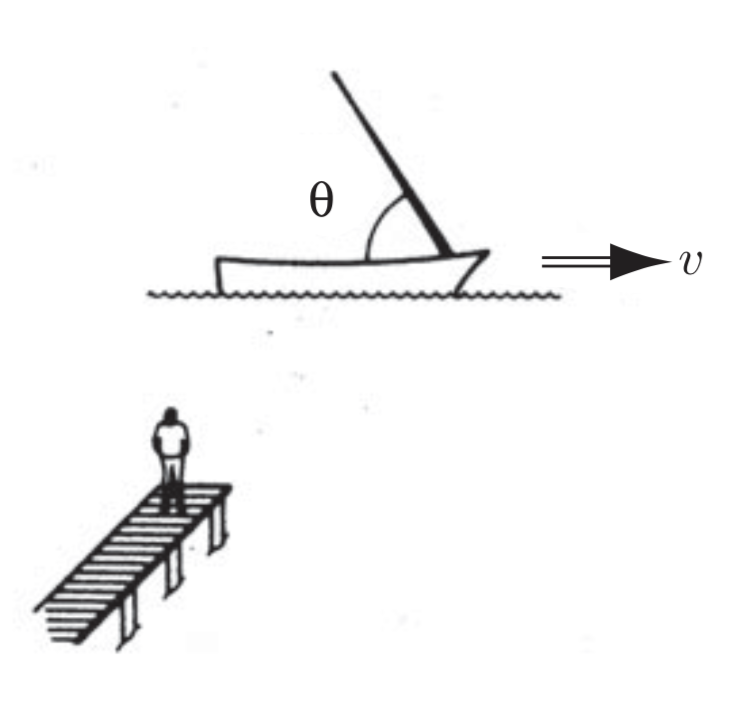
\includegraphics[scale=0.4]{ps11-pic1.png}
\end{center}

{\bfit{Solution}} \\ 

If the length of the mast at rest is $\bar l$, the mast has a vertical component $\bar l_v = \bar l \sin\bar\theta$ and a horizontal component $\bar l_h = \bar l \cos\bar\theta$. Since the boat is travelling in the direction parallel to the horizontal component, only this component will undergo Lorentz contraction in the observer's frame, as follows:

$$l_h = \frac{\bar l\cos\bar\theta}{\gamma}$$ \ 

Since the vertical component is unaffected, the observer will ``see" the following angle $\theta$:

$$\tan\theta = \frac{\bar l \sin\bar\theta}{\frac{\bar l\cos\bar\theta}{\gamma}} = \frac{\gamma \bar l \sin\bar\theta}{\bar l\cos\bar\theta} = \gamma \tan\bar\theta$$ 

$$\therefore \;\; \theta = \tan^{-1}(\tan\bar\theta)$$ \ 




 

\hrulefill 

\hfill 

{\LARGE \bf VI --- Doppler Effect} \\ 

{\Large \bf a.} Prove the formula for the relativistic Doppler effect when the light source approaches the receiver with speed $v$, given by:

$$\nu = \sqrt{\frac{1+\beta}{1-\beta}} \nu_0$$ \ 

where $\nu_0$ is the emitted frequenecy in the source's frame, $\nu$ is the observed frequency in the receiver's frame, and $\beta = \frac vc$. {\it Hint:} start with the wavelength in the receiver's frame given by:

$$\lambda = \frac{cT - vT}{n}$$ \ 

where $cT - vT$ is the length extent of the waves in the receiver's frame and $n$ is the number of pulses emitted over time interval $T$ in the receiver's frame. Also, consider that the number of pulses $n = \nu T$ should be invariant in both frames. \\ 

{\bfit{Solution}} \\ 

Since the source is moving at velocity $v$, after emits one maximum, it moves a distancee $vT$ towards the receiver before it emits the next maximum. The two successive maxima will be $\lambda = cT-vT$ apart. The second maximum will arrive with period:

$$T = \frac \lambda c - \frac{c-v}{c} T_0$$ \ 

where $T_0$ is the period in the source's frame. The frequency in the receiver's frame is thus:

$$\nu = \frac{1}{T} = \bigg(\frac{c}{c-v} \bigg) \frac 1T = \frac{1}{\big( 1-\frac vc \big)} \frac{1}{T} = \frac{1}{\big( 1-\frac vc \big)} \frac{1}{\gamma T_0}$$ \

And, since $T_0 = \frac{1}{\nu_0}$:

$$
\begin{aligned}
	\nu &= \frac{1}{\big( 1-\frac vc \big)} \frac 1\gamma \nu_0 \\ 
	&= \frac{\sqrt{1-\frac{v^2}{c^2}}}{\big( 1-\frac vc \big)} \nu_0 \\ 
	&= \frac{\sqrt{(1-\frac{v^2}{c^2})(1+\frac{v^2}{c^2})}}{\big( 1-\frac vc \big)} \nu_0 \\
	&= \sqrt{\frac{1+\frac vc}{1-\frac vc}} \nu_0 
\end{aligned}
$$ \ 

and, since $\beta = \frac vc$:

$$\nu =\sqrt{\frac{1+\beta}{1-\beta}} \nu_0$$ \ 






\dotfill 

\hfill 

{\Large \bf b.} A spaceship moves radially away from earth with acceleration 25 m/s$^2$. How long does it take for the sodium lamp ($\lambda \simeq 589$ nm) on earth to be invisible (with a powerful telescope) to the human eye of the astronauts? The range of visible wavelengths is about 400-700 nm. \\ 

{\bfit{Solution}} \\ 

Noting the following relationship:

$$\frac{\nu}{\nu_0} = \frac{\lambda_0}{\lambda} = \frac{589}{700} = 0.8414$$ \ 

Thus, using the formula for the relativistic Doppler effect, 

$$\frac{1+\beta}{1-\beta} = 0.8414^2$$

$$\Longrightarrow \; \; \beta = 0.171$$ \

The time taken is: 

$$t = \frac va = \frac{0.171c}{25} = 2.052\cdot 10^6 \; \text s$$ \  

\end{multicols*}

\end{document}
